The storage station is a shelf of ten drawers and is constructed entirely from aluminum profiles.
At the heart of the storage box are the modular drawers, which consist of a universal basic
construction and individual sheet metal part support plates. The basic construction consists
of an aluminum profile frame, two telescopic rails and a locking mechanism, which prevents the
drawer from moving unintentionally when pulled out or pushed in. Due to the greater need for profiles and
connection technology, the costs for this construction method are somewhat higher, but the storage
box can be manufactured precisely as a result, which will have a positive effect on process reliability
later when the sheet metal parts are stored.

\begin{figure}[h]
    \centering
    \begin{subfigure}{0.35\textwidth}
        \centering
        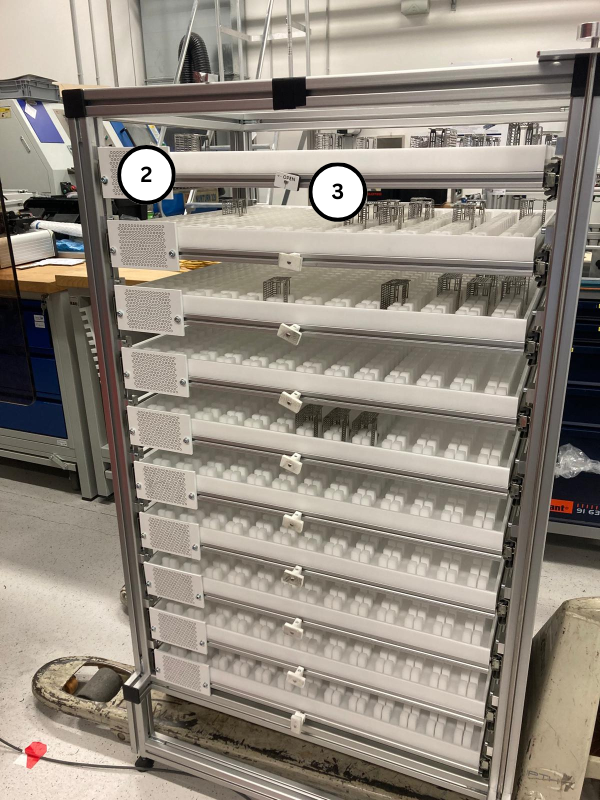
\includegraphics[width=\textwidth]{figures/storage-station-front.png} % Replace with your image file
        \subcaption{front-view}
        \label{fig:storage-station-front}
    \end{subfigure}\hspace{1cm}
    \begin{subfigure}{0.36\textwidth}
        \centering
        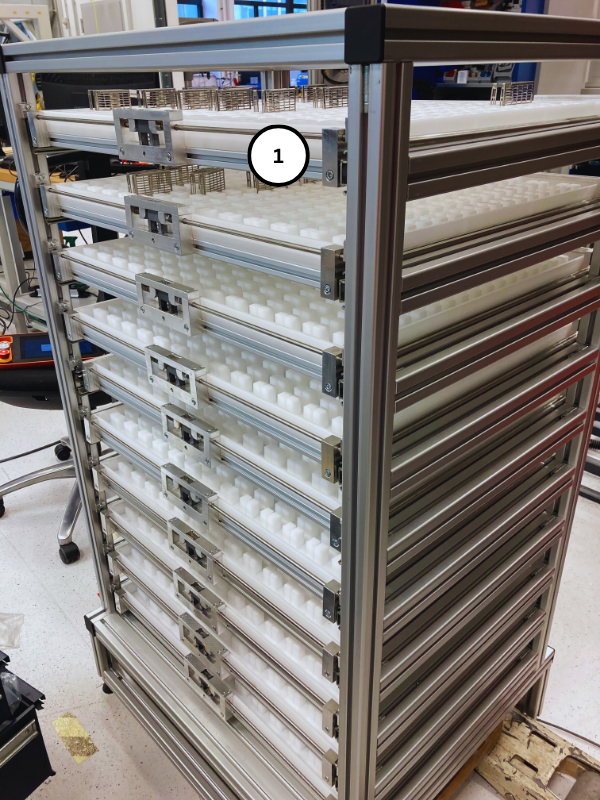
\includegraphics[width=\textwidth]{figures/storage-station-back.png} % Replace with your image file
        \caption{back-view}
        \label{fig:storage-station-back}
    \end{subfigure}
    \caption{Storage station of ten drawers 1) drawer 2) marker 3) shelf handle}
    \label{fig:storage-station-main}
\end{figure}

The individual drawers could be pulled out using
telescopic rails automatically by the robot. 
The individual drawer is a 30 mm thick plate with regularly arranged recesses,
which enables the finished sheet metal parts to be placed in a defined position for the robot unit. For
weight reasons, plastic was the only material considered and the drawers are printed using \hyperref[acro:AM]{AM}.
Due to the possibility of customizing the sheet metal part carrier plate, the
focus of the design implementation was on designing a carrier plate that can be used for several sheet
metal part variants at the same time. On the one hand, this saves material resources, and on the other
hand, different sheet metal part carrier plates do not have to be kept in stock or the storage boxes do
not always have to be converted when changing products.


Each drawer has its own locking mechanism. This is operated with a handle on the front by turning it
clockwise or anticlockwise. The handle also serves as a gripping object for the robot
unit, by means of which the drawer can be pulled out or pushed in. In addition to this locking mechanism,
each storage box has a locking bar across all drawers. This is intended to serve as an additional
safeguard when the boxes are moved between different factory halls and/or over longer distances
using a forklift truck. In addition, each individual drawer is equipped with a detection marker pattern that is
used to determine the spatial position using the camera on the robot unit. This is required
for the reliable depositing of the sheet metal parts.